\documentclass[12pt,twoside,english]{article}
\usepackage[utf8]{inputenc}

%%%%%%%%%%%%%%%%%%%%%%%%%%%%%%%%%%%%%%%%%%%%%%%%%%%%%%%%%%%%%%%%%%%%%%%
%% template for II2202 proposal
%% original 2020.08.28
%% revised  
%%%%%%%%%%%%%%%%%%%%%%%%%%%%%%%%%%%%%%%%%%%%%%%%%%%%%%%%%%%%%%%%%%%%%%%
%

%%% Local Variables:
%%% mode: latex
%%% TeX-master: "."
%%% End:

%%TC:ignore
\usepackage[paper=a4paper,dvips,top=1.5cm,left=1.5cm,right=1.5cm,
    foot=1cm,bottom=1.5cm]{geometry}


\usepackage{todonotes}          %to provide inline and margin notes
%\usepackage[T1]{fontenc}
%%\usepackage{pslatex}
\renewcommand{\rmdefault}{ptm} 
\usepackage{mathptmx}
\usepackage[scaled=.90]{helvet}
\usepackage{courier}
%
\usepackage{bookmark}

\usepackage{fancyhdr}
\pagestyle{fancy}

%%----------------------------------------------------------------------------
%%   pcap2tex stuff
%%----------------------------------------------------------------------------
 %%\usepackage[dvipsnames*,svgnames]{xcolor} %% For extended colors
 %%\usepackage{tikz}  %% Already loaded
 %%\usetikzlibrary{arrows,decorations.pathmorphing,backgrounds,fit,positioning,calc,shapes}

%% \usepackage{pgfmath}	% --math engine
%%----------------------------------------------------------------------------
%% \usepackage[latin1]{inputenc}
\usepackage[utf8]{inputenc} % inputenc allows the user to input accented characters directly from the keyboard
\usepackage[english]{babel}
%% \usepackage{rotating}		 %% For text rotating
\usepackage{array}			 %% For table wrapping
\usepackage{graphicx}	                 %% Support for images
\usepackage{float}			 %% Suppor for more flexible floating box positioning
\usepackage{color}                       %% Support for colour 
\usepackage{mdwlist}
%% \usepackage{setspace}                 %% For fine-grained control over line spacing
%% \usepackage{listings}		 %% For source code listing
%% \usepackage{bytefield}                %% For packet drawings
\usepackage{tabularx}		         %% For simple table stretching
%%\usepackage{multirow}	                 %% Support for multirow colums in tables
\usepackage{dcolumn}	                 %% Support for decimal point alignment in tables
\usepackage{url}	                 %% Support for breaking URLs
\usepackage[perpage,para,symbol]{footmisc} %% use symbols to ``number'' footnotes and reset which symbol is used first on each page
\usepackage[binary-units=true]{siunitx} %% to be able to use binary units
\newcommand{\SIadj}[2]{\SI[number-unit-product={\text{-}}]{#1}{#2}}

%% \usepackage{pygmentize}           %% required to use minted -- see python-pygments - Pygments is a Syntax Highlighting Package written in Python
%% \usepackage{minted}		     %% For source code highlighting

%% \usepackage{hyperref}		
\usepackage[all]{hypcap}	 %% Prevents an issue related to hyperref and caption linking
%% setup hyperref to use the darkblue color on links
%% \hypersetup{colorlinks,breaklinks,
%%             linkcolor=darkblue,urlcolor=darkblue,
%%             anchorcolor=darkblue,citecolor=darkblue}

%% Some definitions of used colors
\definecolor{darkblue}{rgb}{0.0,0.0,0.3} %% define a color called darkblue
\definecolor{darkred}{rgb}{0.4,0.0,0.0}
\definecolor{red}{rgb}{0.7,0.0,0.0}
\definecolor{lightgrey}{rgb}{0.8,0.8,0.8} 
\definecolor{grey}{rgb}{0.6,0.6,0.6}
\definecolor{darkgrey}{rgb}{0.4,0.4,0.4}
%% Reduce hyphenation as much as possible
\hyphenpenalty=15000 
\tolerance=1000

%% useful redefinitions to use with tables
\newcommand{\rr}{\raggedright} %% raggedright command redefinition
\newcommand{\rl}{\raggedleft} %% raggedleft command redefinition
\newcommand{\tn}{\tabularnewline} %% tabularnewline command redefinition

%% definition of new command for bytefield package
\newcommand{\colorbitbox}[3]{%
	\rlap{\bitbox{#2}{\color{#1}\rule{\width}{\height}}}%
	\bitbox{#2}{#3}}

%% command to ease switching to red color text
\newcommand{\red}{\color{red}}
%%redefinition of paragraph command to insert a breakline after it
\makeatletter
\renewcommand\paragraph{\@startsection{paragraph}{4}{\z@}%
  {-3.25ex\@plus -1ex \@minus -.2ex}%
  {1.5ex \@plus .2ex}%
  {\normalfont\normalsize\bfseries}}
\makeatother

%%redefinition of subparagraph command to insert a breakline after it
\makeatletter
\renewcommand\subparagraph{\@startsection{subparagraph}{5}{\z@}%
  {-3.25ex\@plus -1ex \@minus -.2ex}%
  {1.5ex \@plus .2ex}%
  {\normalfont\normalsize\bfseries}}
\makeatother

\setcounter{tocdepth}{3}	%% 3 depth levels in TOC
\setcounter{secnumdepth}{5}
%% Acronyms
\usepackage[acronym, nopostdot]{glossaries}
\glsdisablehyper
\makeglossaries

\renewcommand{\headrulewidth}{0pt}
%%%%%%%%%%%%%%%%%%%%%%%%%%%%%%%%%%%%%%%%%%%%%%%%%%%%%%%%%%%%%%%%%%%%
%% End of preamble
%%%%%%%%%%%%%%%%%%%%%%%%%%%%%%%%%%%%%%%%%%%%%%%%%%%%%%%%%%%%%%%%%%%%

\newacronym{AR}{AR}{augmented reality}

\title{Trade-offs Between Immersion and Energy Consumption With Automatic Naturalistic Lighting in Augmented Reality}
\author{
        \textsc{Stefano Formicola}
            \qquad
        \textsc{Christoph Albert Johns}
        \mbox{}\\
        \normalsize
            \texttt{formico}
        \textbar{}
            \texttt{cajohns}
        \normalsize
            \texttt{@kth.se}
}
\date{\today}


\lhead{II2202, Fall 2020, Period 1-2}
%% or \lhead{II2202, Fall 2020, Period 1}
\chead{Research Plan}
\rhead{\date{\today}}

\makeatletter
\let\ps@plain\ps@fancy 
\makeatother

\setlength{\headheight}{15pt}
\begin{document}

\maketitle


% \begin{abstract}
% \label{sec:abstract}

% Your abstract here.

% \end{abstract}
%%\clearpage

\selectlanguage{english}

\section{Introduction}
\label{sect:introduction}

This research aims at illuminating the relationship between immersion and energy impact in deploying advanced \gls{AR} features, thus empowering developers and designers to decide the most appropriate feature sets for their applications considering both user experience and sustainability aspects.


\section{Project organization}
\label{sect:organization}

The research project will be conducted as a two-person project on the basis of previously published work in the domains of user-based studies on immersion in video games and technology-centric research on virtual lighting in \gls{AR} scenes.

Stefano Formicola is responsible for collecting data during the experiment, writing the sections regarding research questions, method, results, and discussion in the final report, and presenting the project plan.
Christoph Albert Johns is responsible for providing the test application, writing the abstract and sections on introduction and literature study for the final report, as well as preparing and giving the final presentation.

The related literature -- primarily Jennett et al.~\cite{jennett_measuring_2008} -- will provide guidance on how to gather data relating to participants' subjective experience and more specifically immersion, while Apple's Developer Tools will provide access to device-specific measures and more specifically energy consumption levels.
Once the test application is ready to be used, data collection and analysis will proceed in parallel.


\section{Background}
\label{sect:background}
The proposed research project builds on two main lines of research: prior works evaluating the relationship between visual characteristics of \gls{AR} objects and user experience (e.g.~\cite{gabbard_effects_2006}) and research on the approximation of natural lighting conditions within virtual scenes in augmented reality (e.g.~\cite{aittala_inverse_2010}).
While there has been extensive research on the effect of design decisions on several aspects of user experience in digital games~\cite{johnson_validation_2018} -- even in \gls{AR} games in a few instances (e.g.~\cite{georgiou_development_2017}) -- the effect of lighting and more specifically automatic naturalistic lighting in \gls{AR} games on immersion seems not to have been examined yet.

To achieve naturalistic lighting, camera-sensor data is used to estimate and approximate the environment's lighting conditions and dynamically add the appropriate shading to the objects in a scene~\cite{apple_arlightestimate_nodate,apple_pointlight_nodate}.
Depending on the scene and lighting conditions, this can be a computationally intensive process~\cite{steed_constructing_2016}.

With automatic naturalistic lighting becoming increasingly available and common, for example through Apple's RealityKit API~\cite{apple_realitykit_nodate}, it remains unclear whether this feature should be deployed by developers to enhance immersion -- especially since it could strongly affect energy consumption.

While several aspects of the experience when playing videos games in general and \gls{AR} games in particular have been defined and measured as well (see~\cite{dey_systematic_2018, dunser_survey_2008} for overviews), we chose to investigate the effect of automatic naturalistic lighting on immersion because -- in contrast to, for example, \textit{flow}~\cite{csikszentmihalyi_flow_1990} -- it is independent from optimal experience, which our method will not be able to produce, and very likely to relate to visual presentation and, therefore, lighting~\cite{jennett_measuring_2008}.
As Witmer and Singer argue, "scene realism" is one of the governing factors for presence in virtual environments~\cite{witmer_measuring_1998}, which in turn affects how immersive a virtual environment appears~\cite{jennett_measuring_2008}.
We reason that automatic naturalistic lighting enhances this sense of realism and will therefore affect users' sense of immersion.

\section{Problem statement}
\label{sect:problem_statement}

The project will propose and evaluate a method to investigate whether there is a trade-off between an increased energy impact and higher levels of immersion through the use of possibly computationally intensive environment light probing and estimation in \gls{AR} scenes.
To achieve naturalistic virtual lighting, video from the \gls{AR} system's camera feed is continuously probed at a high frequency to estimate the environment lighting conditions~\cite{apple_adding_nodate}.
These estimates are then used as input data for the applied shading algorithms~\cite{apple_adding_nodate}.
This could lead to increased scene realism at the cost of decreased energy efficiency.
While there have been user-based studies evaluating visual characteristics of \gls{AR} objects, this particular aspect of automatic naturalistic lighting appears not to have been examined yet.

\section{Problem}
\label{sect:problem}

Examining the problem statement, two eventual outcomes of our project are possible:
if we find a trade-off between immersion and energy consumption, designers and developers should be recommended to avoid continuous \gls{AR} light estimation in order to free resources for either alternative uses or to extend battery life.
If we find no trade-off, developers and designers can be responsibly encouraged to implement features that enhance immersion.
Each outcome could be considered a worthwhile contribution to the field of \gls{AR} and immersion research.

In this project, immersion will be measured via the \gls{IEQ}~\cite{jennett_measuring_2008}.
Energy consumption will be measured in terms of \gls{CPU} usage for two major reasons.
First, because there is no dedicated \gls{GPU} in the mobile devices we will be testing, so the \gls{CPU} will handle all processing related to the \gls{AR} experience.
And second, because CPU usage can very finely be measured on the test device in contrast to general energy consumption.

Overall, we will explore the following questions:

\begin{description}
    \item[RQ1.] Do users perceive a difference in immersion between enabled and disabled automatic naturalistic lighting?
    \item[RQ1a.] If they perceive a difference, are the participants able to tell that lighting is the cause?
    \item[RQ2.] How does enabling automatic naturalistic lighting affect \gls{CPU} usage?
\end{description}

\section{Hypotheses}
\label{sect:hypotheses}

The main metrics we will collect for each of the two conditions are immersion level and \gls{CPU} usage.
Immersion will be measured once after each run through the \gls{IEQ}, \gls{CPU} usage will be measured over time through Xcode's Developer Tools.
While we are aware that we will only be able to test the proposed method on a small scale, we hypothesize the following outcomes for a full-scale experiment.

As described in section \ref{sect:background}, scene realism is positively correlated with presence and thereby immersion.
That is why we expect the lighting condition that more closely matches the scene's natural environment to lead to higher levels of immersion, resulting in the following hypothesis:

\begin{description}
    \item[H1.] Users experience higher immersion levels when automatic naturalistic lighting is enabled.
\end{description}

Because the difference between both conditions lies in a salient visual feature which affects \gls{AR} objects' color and reflections, we expect not only the indirect measure of immersion as assessed through the \gls{IEQ} to be affected.
We instead hypothesize that users will recognize the difference between both conditions and will be able to articulate how they differ without support from the examiner.
This leads us to this hypothesis:

\begin{description}
    \item[H1a.] Users are able to tell that the lighting was different between both runs of the experiment.
\end{description}

Finally, regarding the energy impact of naturalistic lighting, we expect the computationally intensive continuous probing and estimation of the \gls{AR} scenes environment lighting to lead to higher levels of overall \gls{CPU} usage:

\begin{description}
    \item[H2.] \gls{CPU} usage is higher when automatic naturalistic lighting is enabled.
\end{description}





\section{Goal}
\label{sect:goals}

The goal of this project is to propose and pretest a method for exploring the relationship between immersion and energy impact when deploying automatic naturalistic lighting using a simple example application and an existing \gls{AR} \gls{API}.

The expected deliverables and outcomes are: an example \gls{AR} application to measure immersion levels and monitor energy consumption; a pre-tested and evaluated method (setup, procedure, and analysis) for a full-scale study; an indication for the results of a full-scale study.

\section{Tasks}
\label{sect:tasks}

We will modify an existing \gls{AR} mobile game based on player concentration as a sample application to test immersion levels and energy consumption during usage.
Because of its popularity across countries and languages, we consider the game \textit{Memory} or \textit{Concentration}, in which players have to remember the order and color of different cards, a valid candidate for the experiment.

The implementation will be done for iOS devices and developed on Apple's \gls{IDE} Xcode using the ARKit and RealityKit frameworks.
The user interface will include a toggle button invisible to the player that enables and disables the automatic naturalistic lighting feature for the two runs of the experiment.

The experiment will consist of one three-minute session of gameplay for each condition, with and without the automatic naturalistic lighting, per subject.
During each phase of the experiment a non-invasive data collection will be performed using Xcode Developer Tools' \emph{Instruments} to measure the computational load.

Finally, we will measure subjects' immersion levels for each condition using the \gls{IEQ} proposed by Jennett et al.~\cite{jennett_measuring_2008}.

\section{Method}
\label{sect:method}

The project will use a within-subjects design to empirically test two different lighting conditions in an experiment setting and analyze the results using statistical methods.
In the following, the targeted participant profile as well as study procedure, data collection, and data analysis will be described.

\subsection{Participants}
\label{sect:participants}

Participants will be recruited via an opportunity sample and will -- due to the difficulties and restrictions regarding gatherings of people during the COVID-19 pandemic -- mostly be international students living at KTH Main Campus between 19 and 30 years old.
To limit the effect of novelty on immersion levels, participants should have had played a card-matching game similar to the sample game before.
It is, however, not required that they have played a digital version of this game before taking part in the experiment.
To further mitigate the effect of novelty, participants should have experienced an \gls{AR} scene on a mobile handheld device before.
Due to above reasons and the limited time available for recruitment, we expect around ten participants to take part in the small-scale study of this project.

\subsection{Procedure}
\label{sect:procedure}

We will modify an open-source \gls{AR} card-matching game~\cite{cobb_maxxfrazerrealitykit-cardflip_2020} to include an option to enable and disable automatic naturalistic lighting using RealityKit's \textit{.disableAREnvironmentLighting} render option for a repeated measures study design.
The sample game will be presented to participants on an Apple iPad in an indoor setting with controlled lighting where participants will be asked to complete as many rounds of the card-matching game for each of the two lighting conditions as they can, before they are interrupted after three minutes and the render option is changed for the second run.
The order of render options will be randomized to improve reliability.
The purpose of the experiment will be stated to the participants only in general terms as "investigating immersion in \gls{AR} games" to avoid influencing their perception of the scene by directing their attention towards lighting.
Participants will not be informed about the currently active render option for the same reason.
The sample application has been chosen due to its simplicity in functionality and visual presentation as well as general familiarity, thereby reducing the risk of errors in use or unwanted effects on immersion due to scene complexity or novelty.
To further negate this risk and to address the concerns brought up by Jennett et al.~\cite{jennett_measuring_2008} regarding the effect of prior experience on immersion, participants will be given a trial period with a third lighting condition: disabled automatic naturalistic lighting and an added point light above the scene.
The goal stated to the participants to complete the game as fast as possible and with as few errors as possible follows the study design of Jennett et al.~\cite{jennett_measuring_2008}.
It should allow for a more challenging experience across player ability levels and, therefore, increase flow~\cite{csikszentmihalyi_flow_1990} and thereby general immersion levels as well as reduce overall variance in immersion~\cite{jennett_measuring_2008}.
The first run will be started, after the participant indicates that they are ready for the experiment to begin.
After the experiment, participants will be debriefed and fully informed about the purpose of the study and given the opportunity to withdraw their consent.
The expected duration of the experiment per participant is 30 minutes.

\subsection{Data collection}
\label{sect:data_collection}

During each run of the experiment, the \gls{IDE} Xcode and more specifically its \textit{Instruments} feature~\cite{apple_xcode_nodate} will be used to log the test device's \gls{CPU} usage according to Apple's type definitions~\cite{apple_system_nodate} in three second intervals.
While there is a more general power metric that can be logged through the same application~\cite{apple_energy_nodate-1}, that metric is discrete and inelastic towards enabled and disabled automatic naturalistic lighting and was, therefore, not used.
We discussed and decided not to have participants think aloud during their app usage to avoid unwanted effects on their experience and, thus, immersion~\cite{van_den_haak_retrospective_2003}.
After each run, participants will be asked to fill out the \gls{IEQ} (see \ref{sect:ieq}) to measure their levels of immersion dependent on the lighting treatment.
After the second run, participants will additionally be asked about their general experience using the application and to elaborate on any differences they noticed between both runs.
While alternatives such as tracking eye movement or measuring reaction times could also be used to measure immersion~\cite{jennett_measuring_2008}, we chose a questionnaire approach as the most economical option that still has satisfactory precedence in literature~\cite{boyle_engagement_2012}.
If a participant mentions one of the words "light", "lighting", "color", or "contrast" while answering these questions, the difference in lighting is considered as noticed by the user.

\subsection{Data analysis}
\label{sect:data_analysis}

After the above data has been successfully gathered, we will conduct a statistical analysis regarding the participants' immersion levels and the \gls{CPU} usage between both lighting conditions using Student's two-sample \textit{t}-test in R to check for significant differences.
We chose this measure as it can be considered quite robust even with small and extremely small ($ N \leq 5 $) sample sizes~\cite{de_winter_using_2013} and because it was used by Jennett et al. in their original experiments~\cite{jennett_measuring_2008}.
If, however, the \textit{t}-test's assumption of normal distribution is not met, we will instead conduct a Mann-Whitney U-test to compare the two conditions following the example of Nordin et al.~\cite{nordin_attention_2013} in their immersion experiments.
Additionally, we will report the results of the interview.

We are aware that both the results of our analysis of variance and the results of our interviews should not be used to infer knowledge about either the effect of automatic naturalistic lighting on immersion or on energy consumption.
Rather, the analysis is carried out in order to evaluate the chosen methods and to illustrate how such analysis should be done if the same study were carried out on a larger scale.

\section{Milestones}
\label{sect:milestones}

The project started on 31 August 2020 and will end at 00:00 on 15 January 2021.
The current status of the project in regards to milestones and deliverables is displayed below.
A graphical representation of the project plan as displayed in the project proposal can be found in Appendix \ref{sect:gantt_chart}.

\begin{description}
\item{Sep 16} Delivered the project plan and started work on the Ethics \& Sustainability document

\item {Sep 18} Delivered presentation of reflections on Ethics \& Sustainability of the proposed research

\item {Oct 6} Ended the first phase of literature study started at the beginning of the project; finalized modification of the mobile application needed for the experiment; set up Google Form for gathering data from participants using the \gls{IEQ}

\item {Oct 9} Presentation of the Research Plan and setup of the tools needed for the experiment

\item {Oct 12} The Experimentation and its data collection will start

\item {Nov 20} All data will be collected

\item {Nov 27} All data will be analyzed

\item {Nov 30} First draft of the Final Report

\item {Jan 15} Deliver of the final report, improved version of the first draft, and its presentation

\end{description}

\section{Risks}
\label{sect:risks}
The major risks of executing the proposed research plan lie in participant recruitment and sample app reliability.
As we only have access to limited resources and time to execute the project, recruiting the necessary number of participants for a representative sample to evaluate the hypotheses stated above will be challenging.
That is why we decided to focus on evaluating our proposed method instead and to frame our report around this evaluation as the research contribution, providing the necessary tools and instructions for a full-scale study.
While this does allow for smaller sample size, it will remain challenging to find an appropriate number of willing participants that fit the participant profile.
This risk will be mitigated by allotting a large portion of the total project schedule for recruitment.
The second major risk of sample app reliability refers to the risk of system crashes, lost and unusable data.
Due to the inherent immaturity of the technology used, the modified application is vulnerable to errors, glitches, and crashes.
This has a detrimental effect on both measures of immersion and energy consumption and could, therefore, make entire runs of the experiment unusable for analysis. 
To mitigate this risk, we will implement additional recovery systems that handle app crashes.
Furthermore, we will make use of the remote control features afforded by the Xcode \gls{IDE} to monitor system metrics and intervene in the experiment if necessary.


\bibliography{II2202-proposal}
% \bibliographystyle{IEEEtran}
\bibliographystyle{myIEEEtran}

\appendix
\section{Appendix}
\label{sect:appendix}

\subsection{Immersive Experience Questionnaire}
\label{sect:ieq}
\subfile{lib/ieq}

\subsection{Gantt Chart of the Project Milestones}
\label{sect:gantt_chart}

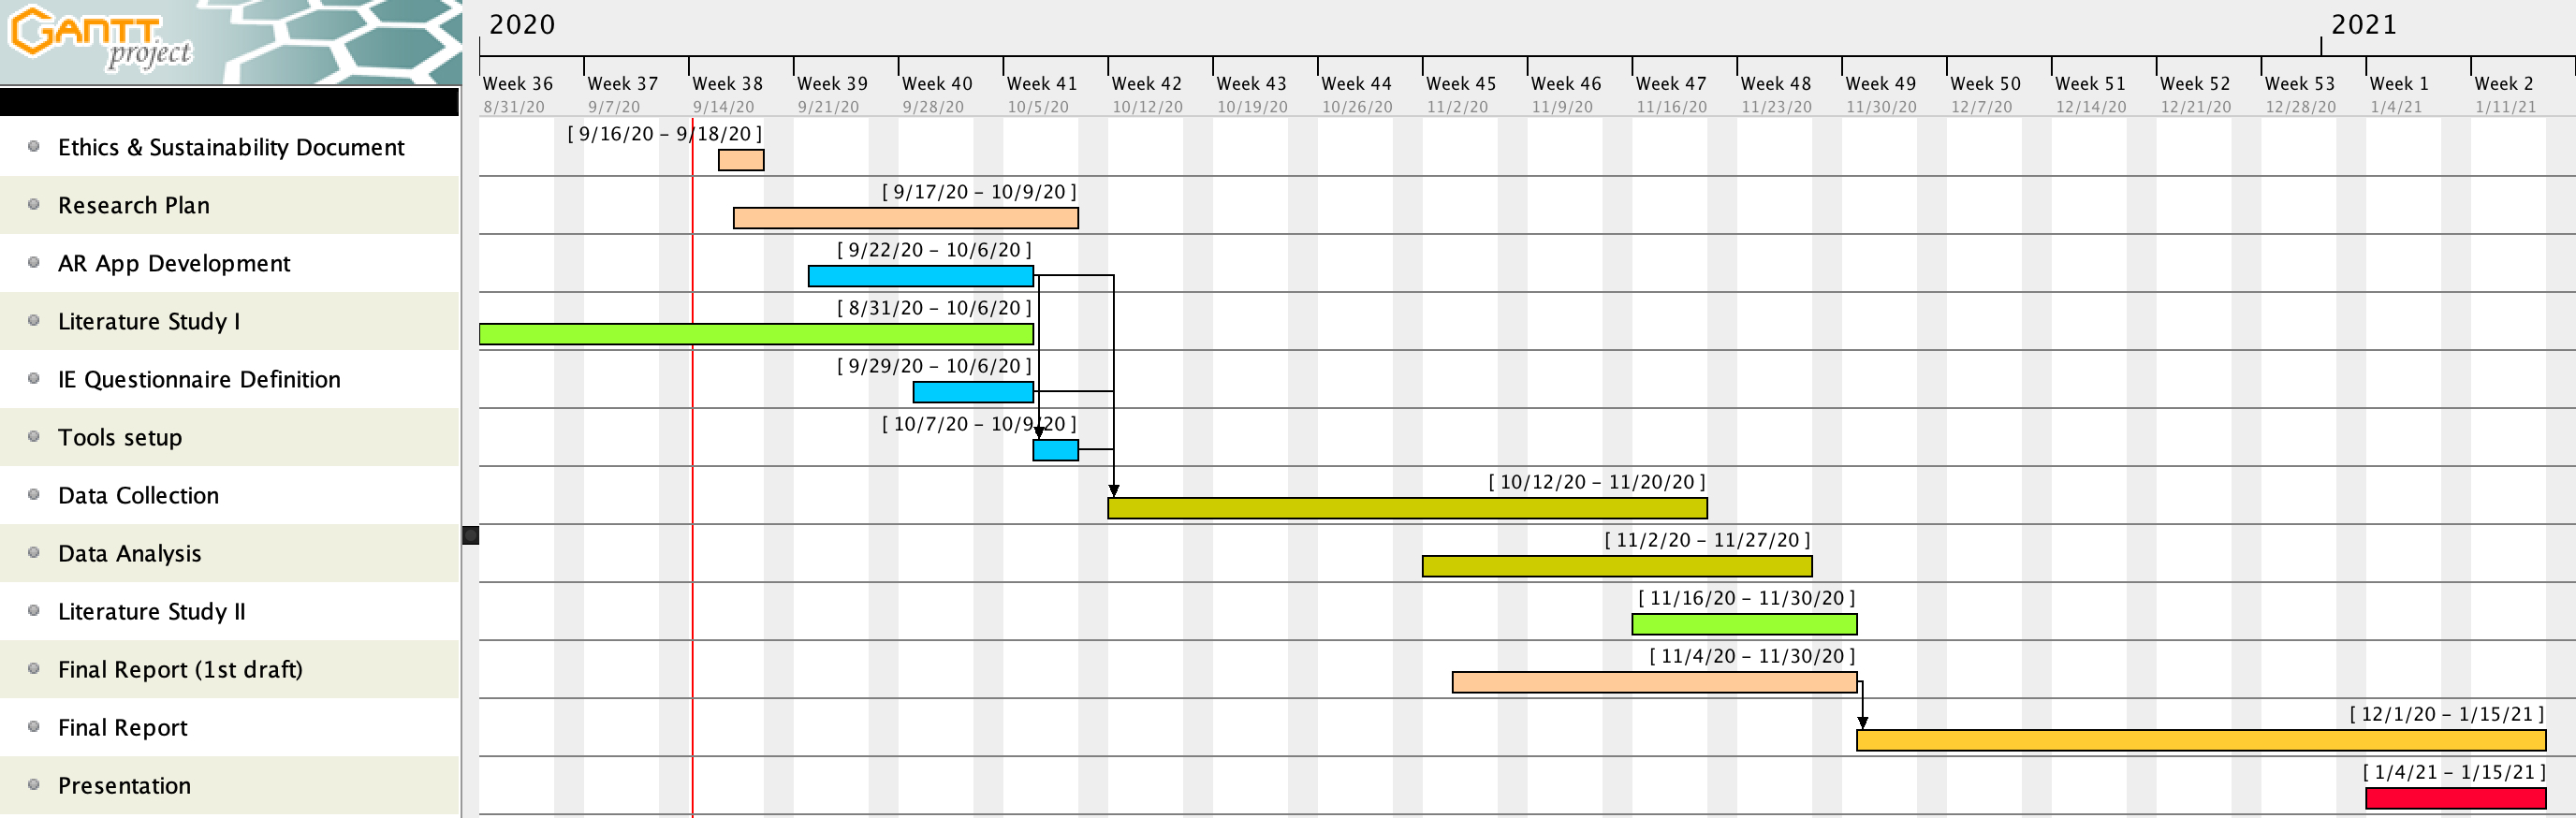
\includegraphics[width=\textwidth]{imgs/project_milestones}

\printglossary[type=\acronymtype, nonumberlist]
\clearpage
\end{document}
